\subsection{Muon triggers}
\label{sec:reco-mu-triggers}

Muons are triggered on at L1 using the RPC in the barrel (\modetalt{1.05}) and
the TGC in the endcaps (\modetalt{2.4}). As shown in~\fig{mu-trigger-diag} the
muon trigger chambers are arranged in three planes of two to four layers. The
trigger is based on coincidences between planes. 
The coverage is $\sim$99\% in the endcaps and $\sim$80\% in the barrel due to
gaps for services and the detector feet.
The RPC planes consist of
doublets of independent layers. For low \pt\ triggers a coincidence in 3 of 4
the four layers of the 2 inner planes is required. The high \pt\ triggers start
from the low \pt\ triggers and look for hits in one of the two layers of the
third layer (referred to as the high \pt\ confirmation plane). Similarly, the two outermost
planes of the TGC consist of doublets of independent detectors and low \pt\
triggers require the coincidence of 3 out of 4 layers of the outer 2 planes. The
inner plane has 3 layers; high \pt\ triggers require coincidences in at least 2
out of 3 layers from innermost plane. Coincidences are generated separately for
$\eta$ and $\phi$; a coincidence is required in both co-ordinates for the
trigger to be fired. To apply a \pt\ threshold to the trigger the coincidences
are required to fall in \int{roads}, parameterised geometrical regions
corresponding to muons of either charge with momentum above a given \pt\
threshold. In 2011 the L1 \pt\ threshold for the primary single muon trigger was
15 \GeV; in 2012 it was 20 \GeV.

The muon HLT uses similar algorithms to the online muon reconstruction described
below. Each L1 muon candidate is refined by including the precision
data from the MDTs and CSCs in the RoI defined by the L1 candidate. MS tracks
are then built by opnening narrow roads around the L1 trigger chamber hits and
associating hits from other chambers to the track. A rough \pt\ measurement is
obtained using a lookup table. The MS tracks are then combined with ID tracks,
reconstructed using the same fast L2 ID tracking as the electron L2 trigger
(see~\sec{reco-el-triggers}).
	- L2 MS-Only - build MS tracks using L1 trigger chamber hits as seeds and opening a narrow road. Track fit using hits and pT addignment from lookup.
	- L2 Combined: combine with ID tracks
	- L2 Isolated: check track and calo iso.At L2 a dedicated fast tracking
algorithm is used. 

- EF:
	- Start from RoI from L2, and run offline algos
	- Outside in: start from L1/L2 RoI and reco MS tracks. then extrapolate to IP and determine para,m there. Then combine with ID track.
	- Inside out - start with ID track and extrapolate to MS
	- 2011, ran both inside out and outside in to maximise efficiency.
	- 2012 - apply isolation at EF ptcone20<0.12  (tracks with pt > 1 and with z_track - z_mu < 6mm
	
2011 to 2012
-------------
Not affected too much by PU, but need to deal with rate
- tighten pt 18 to 24
- add iso
- merge two algo - run outside in first then inside out if it fails.





\begin{figure}[h]
\centering
            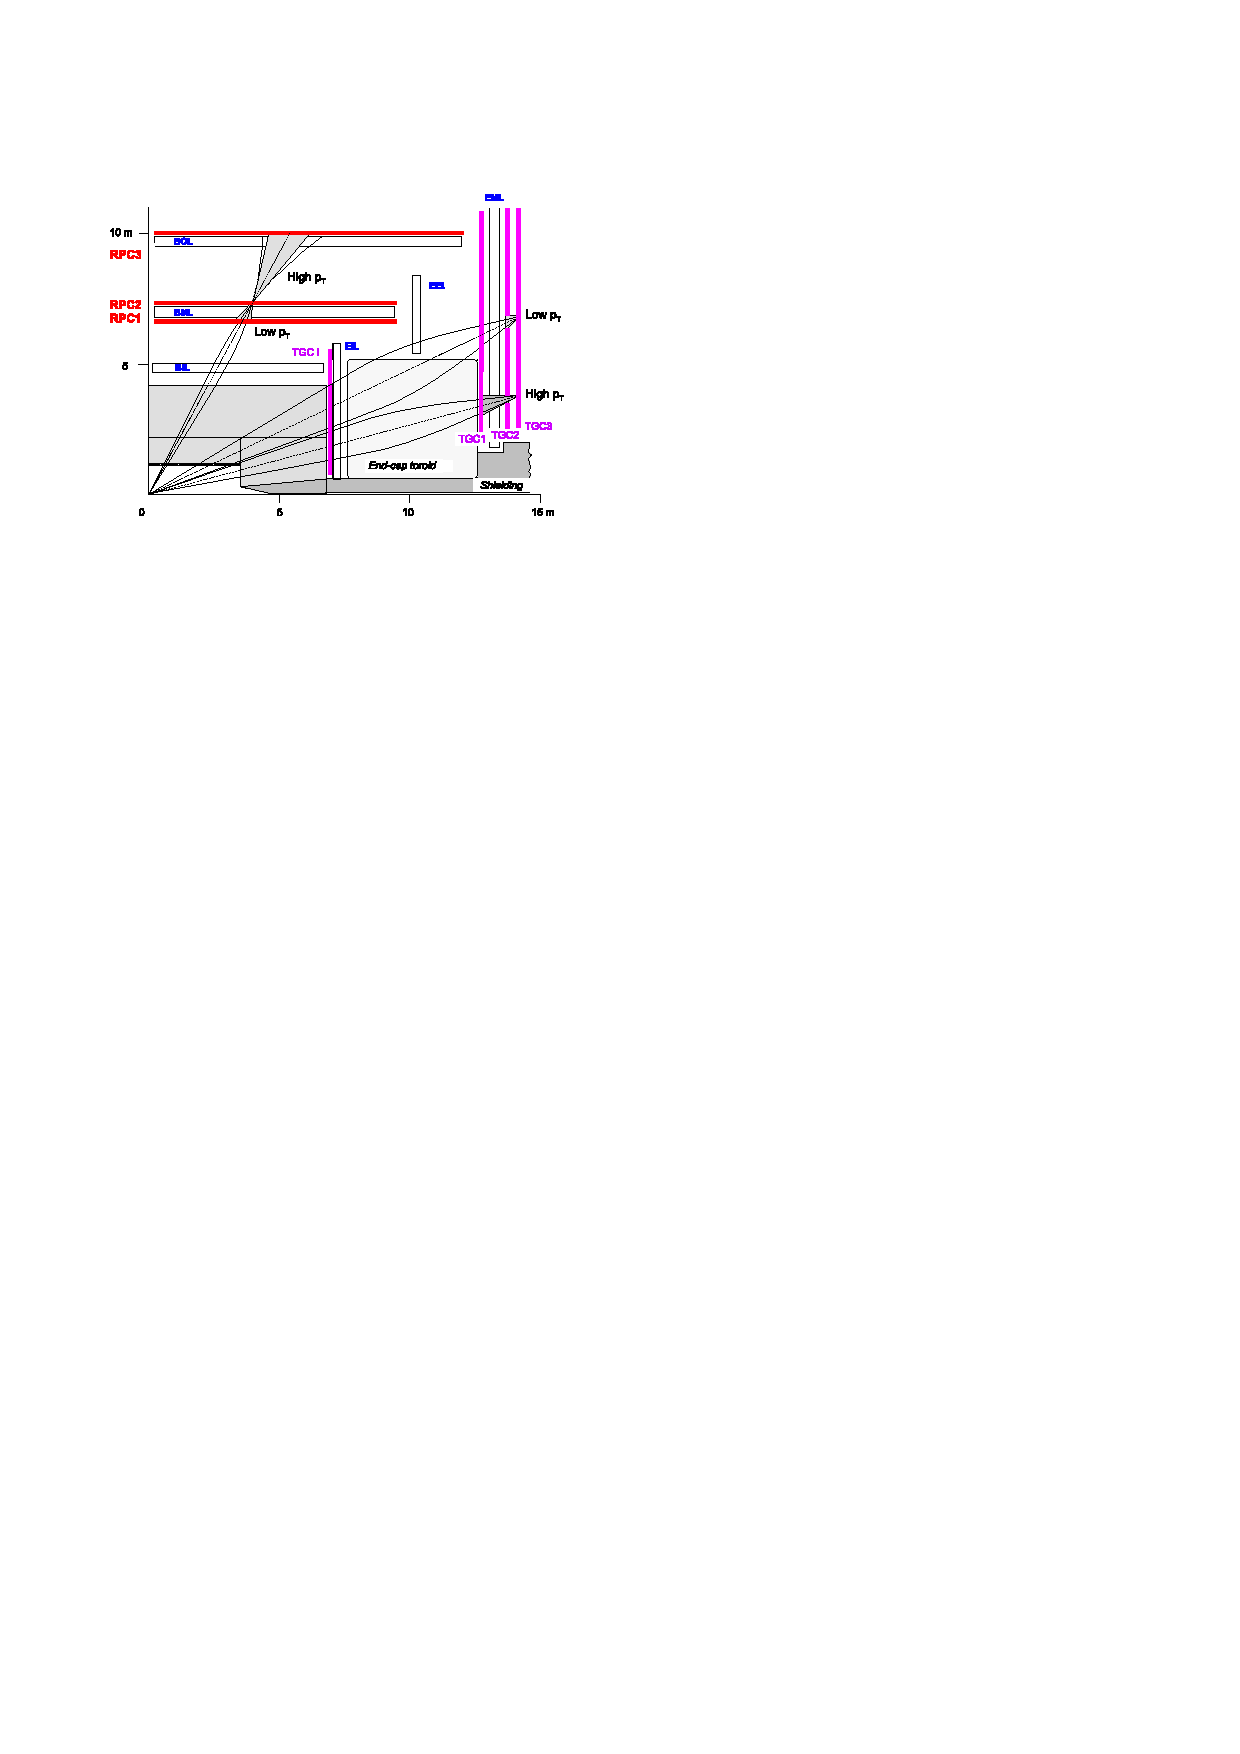
\includegraphics[width=0.8\textwidth]{mu-trigger-diag}
\caption{
Distribution of the Inner Detector material for each sub-detector as a
function of the pseudorapidity. The material of the Pixel and SCT detectors
includes passive material arising from electronics, cabling, cooling and
mechanical support. Figure from~\cite{2012EPJC...72.1849A}.}
\label{fig:mu-trigger-diag}
\end{figure}

- Not affected significantly by pileup, but increased lumi requires tightening of pT selection in 2012.
   - 2011: 18 GeV threshold
   - 2012: 24 GeV, plus isolation: ptcone20/pt<12%. Tracks have to have z0<6mm
   


\subsection{Reconstruction and Identification}
\label{sec:reco-el-reco}
